\documentclass[a4paper,11pt]{article}
\usepackage[margin=1.5cm]{geometry}
\usepackage{graphicx}
\usepackage{amsmath}
\usepackage{booktabs}
\usepackage{setspace}
\usepackage{microtype}
\pagenumbering{gobble}

\begin{document}

\begin{center}
\Large\textbf{Is Florida Getting Warmer?}\\[6pt]
\normalsize Permutation Test on Key West Annual Mean Temperature (20th Century)
\end{center}

\vspace{0.5cm}

\section*{1. Methods}
Annual mean temperatures recorded at Key West, Florida, were analyzed for a long-term warming trend.  
We calculated the Pearson correlation coefficient between year and annual mean temperature:
\[
r_{\text{obs}} = 0.5332
\]

Because temperature records over time are not independent, we performed a permutation test:  
the temperature values were randomly reassigned to years \(N = 10000\) times, and the correlation coefficient recalculated each time:
\[
r_i = \text{cor}(\text{Year}, \text{sample(Temp)})
\]

The empirical one-sided p-value is the proportion of permuted correlations greater than or equal to the observed one:
\[
p = \frac{\sum (r_i \ge r_{\text{obs}})}{N} = 0.0000
\]

\section*{2. Results}
The histogram below shows the distribution of correlation coefficients obtained from the permutation test.  
The vertical red line represents the observed correlation \(r_{\text{obs}}\).

\begin{center}
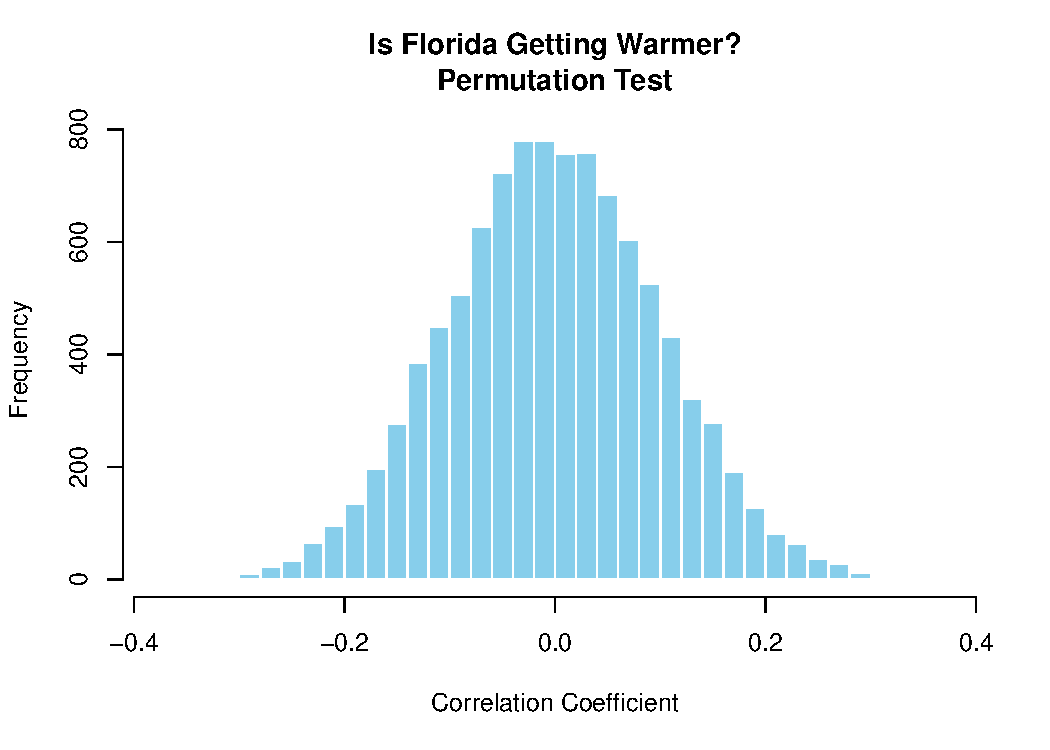
\includegraphics[width=0.9\textwidth]{../results/Florida_histogram.pdf}
\end{center}

\vspace{0.3cm}
\noindent
\textbf{Observed correlation:} \(r = 0.5332\)\\
\textbf{Empirical p-value:} \(p = 0.0000\)\\
\textbf{Number of permutations:} \(N = 10000\)

\end{document}
